\section{SAR影像基础}

\subsection{SAR概述}
\subsubsection{RADAR}
Radar是Radio Detection And Ranging的简写, 一个Radar系统主要包括三个功能:
\begin{itemize}
    \item 发射微波信号到场景
    \item 接收从场景中传回的部分后向散射能量
    \item 观测返回的强度(检测)和延时(测距)信号
\end{itemize}

Radar使用本身的能量源, 因此可以进行全天候观测, 并且可以透过云层覆盖. 这种遥感系统就是主动式遥感系统, 

\subsubsection{SAR}
SAR是Synthetic Aperture Radar的简写, 中文为: 合成孔径雷达. 早期的雷达系统是真实孔径雷达(Real Aperture Radar -- RAR), 由于成像分辨率与雷达天线的长度成正比, 要想得到较高分辨率的SAR图像, 需要增加天线的物理尺寸, 限制其发展和应用. 后来逐渐被合成孔径雷达取代. 

SAR用一个小天线作为单个辐射单元, 将此单元沿一直线不断移动, 在不同位置上接收同一地物的回波信号并进行相关解调压缩处理. 一个小天线通过 ``运动'' 方式就合成一个等效``大天线'', 这样可以得到较高的方位向分辨率, 同时方位向分辨率与距离无关, 这样SAR就可以安装在卫星平台上从而可以获取较高分辨率的SAR图像.

\subsection{SAR重要参数}
\subsubsection{分辨率}
在SAR系统中, 垂直轨道方向的维度叫``距离向—range'', 近方位向边缘最接近天底顶(在雷达垂直方向下的点). 平行轨道方向的维度叫``方位向—azimuth''. 因此, SAR图像分辨率包括距离向分辨率(Range Resolution)和方位向分辨率(Azimuth Resolution), 如图\ref{fig:0101}所示:

\begin{figure}[htbp]
    \centering
    \begin{minipage}{0.4\textwidth}
        \centering
        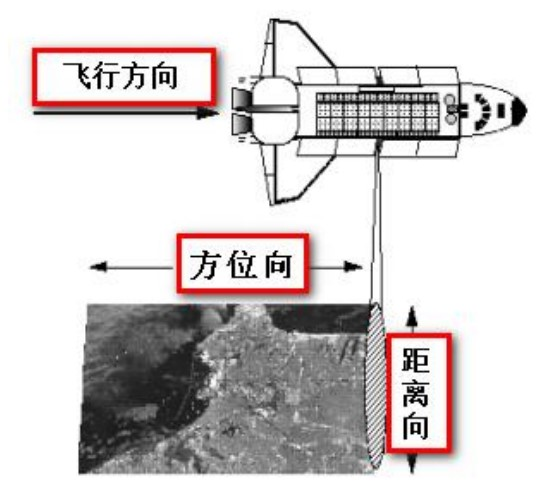
\includegraphics[width=0.8\textwidth]{pic/chap01xx01.jpg}
        \caption{分辨率示意图}
        \label{fig:0101}
    \end{minipage}
    \qquad
    \begin{minipage}{0.4\textwidth}
        \centering
        \begin{tabular}{c c}
            \hline
            波段 &  波长(cm)     \\ \hline
            K波段 & 0.1 - 1.2     \\ \hline
            X波段 & 1.2 - 3.0     \\ \hline
            C波段 & 3.0 - 5.0     \\ \hline
            S波段 & 5.0 - 10.0    \\ \hline
            L波段 & 10.0 - 23.0   \\ \hline
            P波段 & 23.0 - 65.0   \\ \hline
        \end{tabular}
        \caption{波段波长}
        \label{tab:0101}
    \end{minipage}
\end{figure}

距离向分辨率与雷达系统发射的脉冲信号相关, 与脉冲持续时间成正比;SAR系统使用小尺寸的天线也能得到高方位向分辨率, 而且与斜距离无关, 即与遥感平台高度无关.

\subsubsection{波长}
雷达遥感使用的微波部分的电磁频谱, 频率从0.3GHz至300GHz的, 在波长方面, 从1米到1毫米, 如表\ref{tab:0101}所示:

波长越长穿透能力就越强, 如波长大于2cm的雷达系统不会受到云的影响. 小型特征如冰雪识别使用X波段; 大型特征地址制图使用L波段; 叶面渗透最好使用低频率P波段; 一般情况使用C波段. 

\subsubsection{极化}
雷达发射的能量脉冲的电场矢量, 可以在垂直或水平面内被偏振. 无论哪个波长, 雷达信号可以传送水平(H)或者垂直(V)电场矢量, 接收水平(H)或者垂直(V)或者两者的返回信号. 雷达遥感系统常用四种极化方式——HH, VV, HV, VH. 前两者为同向极化, 后两者为异向(交叉)极化.

极化是微波的一个突出特点, 极化方式不同返回的图像信息也不同, 如图\ref{fig:0102}~所示. 返回同极化(HH或者VV)信号的基本物理过程类似准镜面反射, 比如, 平静的水面显示黑色. 交叉极化(HV或者VH)一般返回的信号较弱, 常受不同反射源影响, 如粗糙表面等.

\begin{figure}[htbp]
    \centering
    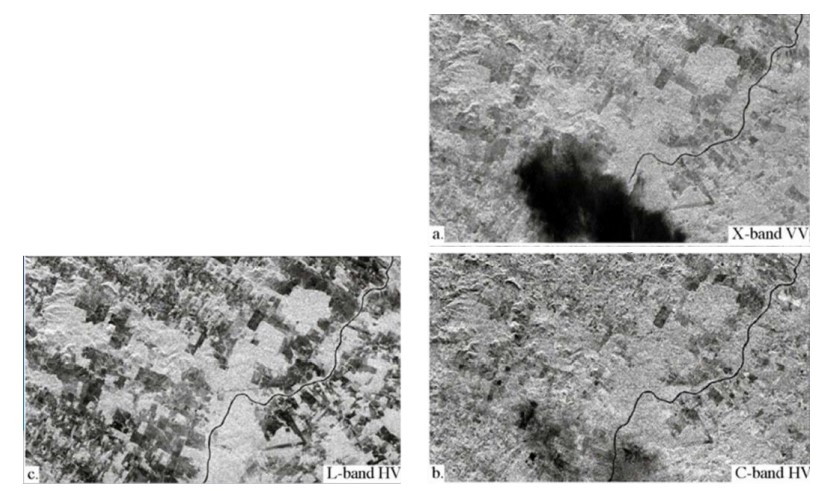
\includegraphics[height=16em]{pic/chap01xx02.jpg}
    \caption{不同极化方式}
    \label{fig:0102}
\end{figure}

\subsubsection{入射角}
入射角也叫视角, 入射角是雷达波束与垂直表面直线之间的夹角, 如图\ref{fig:0103}~所示.

\begin{figure}[htbp]
    \centering
    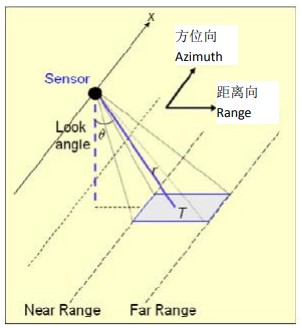
\includegraphics[height=15em]{pic/chap01xx.jpg}
    \caption{入射角}
    \label{fig:0103}
\end{figure}

\begin{itemize}
    \item 微波与表面的相互作用是非常复杂的, 不同的角度区域会产生不同的反射. 
    \item 低入射角通常返回较强的信号, 随着入射角增加, 返回信号逐渐减弱.
\end{itemize}

根据雷达距离地表高度的情况, 入射角会随着近距离到远距离的改变而改变, 依次影响成像几何. 

\subsection{接收模式}
SAR雷达数据获取模式, 不同卫星有多种不同的数据获取模式. 

\subsection{散射}
SAR图像上的信息是地物目标对雷达波束的反映, 主要是地物目标的后向散射形成的图像信息, 即雷达图像表示的是地面雷达后续散射的估算值, 如高亮区域表示高后向散射. 图上高亮要素意味着很大部分的雷达能量反射回雷达系统中.影响后向散射的主要因素分为两大类:
\begin{itemize}
    \item 雷达系统的工作参数: 主要包括雷达传感器的工作波长, 入射角, 极化方式等
    \item 地物目标的特性: 地表的粗糙度和复介电常数等
\end{itemize}

对于特定波长, 一个目标区域的后向散射会受很多条件影响, 如散射体的物理大小, 目标的导电特性, 水分含量等. 主要可分为5种散射: 表面和体散射, 双回波, 组合散射, 渗透散射和介电属性散射.

\subsubsection{表面散射和体散射}
粗糙的表面能得到更高的后向散射, 平整表面在雷达图像上经常表现暗区域. 在大多数波长范围内的雷达系统, 植被表现中规中矩. 如图\ref{fig:0104}~所示:
\begin{figure}[htbp]
    \centering
    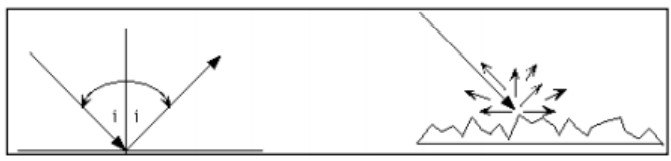
\includegraphics[height=10em]{pic/chap01xx03.jpg}
    \caption{表面散射和体散射}
    \label{fig:0104}
\end{figure}


\subsubsection{双回波}
面向雷达的表面比背向雷达的表面产生更强的后向散射, 如图\ref{fig:0105}~所示, 多在城市的建筑区产生.
\begin{figure}[htbp]
    \centering
    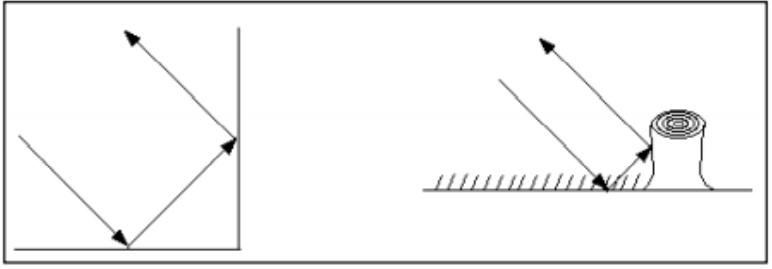
\includegraphics[height=10em]{pic/chap01xx04.jpg}
    \caption{双回波}
    \label{fig:0105}
\end{figure}

\subsubsection{组合散射}
一般发生在低频SAR系统(如L,P波段)包括表面, 体散射, 双回波等, 如图\ref{fig:0106}~所示.
\begin{figure}[htbp]
    \centering
    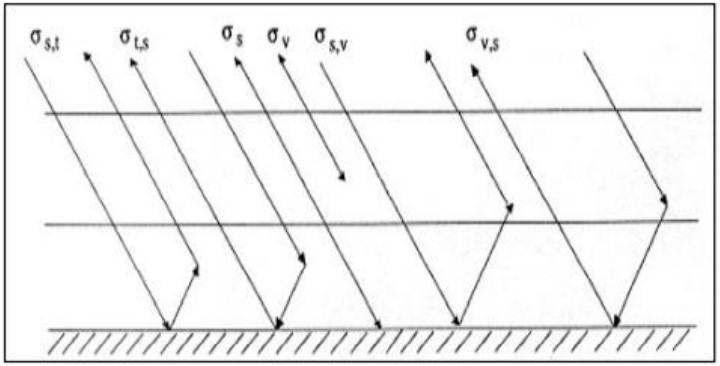
\includegraphics[height=8em]{pic/chap01xx05.jpg}
    \caption{三林的组合散射(上-树冠层, 中-树干层, 下-地面层)}
    \label{fig:0106}
\end{figure}

\subsubsection{渗透散射}
根据极化方式和波长情况, 微波可以透入植被, 裸土(干雪或沙地). 一般情况, 波长越长, 渗透能力越强, 如图\ref{fig:0107}~所示. 交叉极化(VH/HV)相比同极化(HH/VV)的渗透能力弱.
\begin{figure}[!htbp]
    \centering
    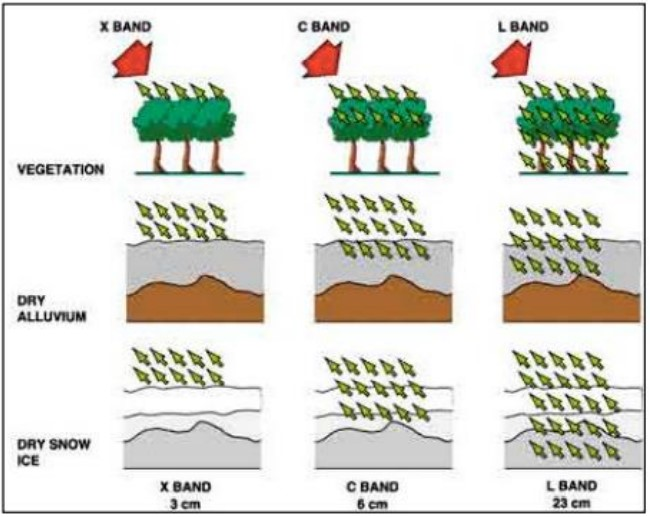
\includegraphics[height=12em]{pic/chap01xx06.jpg}
    \caption{渗透散射}
    \label{fig:0107}
\end{figure}

\subsubsection{介电属性}
目标的介电属性也影响雷达的后向散射. 如金属和水的介电常数很好(80), 而大多数其他材料的介电常数相对较低; 在干燥条件下, 介电常数一般是3~8. 这意味着, 湿润的土壤或植物表面可以产生雷达信号的反射率显着增加. 

基于这种现象, SAR系统也可用于检索土壤水分. 主要原理是基于干土和湿土的介电属性之间的反差. 由于土壤浸湿, 饱和25~30时, 其介电常数变化约2.5. 这相当于增加反射能量. 因此, 从后向散射系数中检测土壤水分是可行的, 为了区分土壤粗糙度和湿度之间的影响, 常使用特定极化和双频率(C, L波段)的SAR传感器.

\paragraph*{雷达参数的影响}

雷达系统的工作参数中的极化方式对雷达波束响应的影响比较大. 一般情况, 自然地物对HH极化产生较强的回波信号, 因此, 地形测绘和资源调查一般选择HH极化SAR图像; 地表比较粗糙(如树木, 农作物等)区域, 回波信号与入射角无关, HH和VV极化方式区别不大; 对于光滑的地面(水体等), HH极化比VV极化回波强度低; 对于建筑物, HH极化的回波强度通常大于VV极化方式; 一般情况, 交叉极化(HV和VH)的回波强度比同极化(HH和VV)低很多. 

\paragraph*{\large\bf 小结}
波长和入射角在上述5种散射类型中有所体现. 如波长可以衡量地表粗糙度, 以及影响复介电常数的不同. 入射角在光滑表面有一些体现, 如海洋雷达图像中, 尽量选择入射角小的图像, 这样能得到回波信号较强的图像. 因此, 地物目标对雷达波束的后向散射作用是很复杂的SAR图像散射特征可以简单归纳为以下几点:
\begin{itemize}
    \item 图像亮度代表后向散射强度
    \item 像元内表面越粗糙, 后向散射越强
    \item 光滑表面镜面反射, 后向散射很弱
    \item 与散射体的复介电常数有关, 含水量越大, 后向散射越强
\end{itemize}

\subsection{斑点}
\begin{itemize}
    \item SAR是相干系统, 斑点噪声是其固有特性
    \item 均匀的区域, 图像表现出明显的亮度随机变化, 与分辨率, 极化, 入射角没有直接关系, 属于乘机噪声
    \item 多视和滤波可以抑制斑点噪声
\end{itemize}


\subsection{数据类型}
分为SLC数据与GRD数据. SLC(Single Look Complex)数据是指单视复数影像, 包含相位信息, 相位信息可以用来研究相干性和干涉特性; GRD(Ground Range Detected)数据是指地距多视影像, 不包括相位信息.

\subsection{SAR成像几何}
由于合成孔径雷达图像数据在距离向和方位向方面具有完全不同的几何特征, 可以考虑将其成像几何特征分离开来理解. 根据成像几何特征的定义, 在距离向的变形比较大, 主要是由地形变化造成的, 在方位向的变形则更小但更为复杂. 

距离向的比例尺由地面目标到雷达天线的距离决定. 在距离向上, 离 SAR越近, 变形就越大, 这跟光学遥感图像刚好相反. 距离向上分为两种投影, 如图\ref{fig:0108}~所示:
\begin{figure}[htbp]
    \centering
    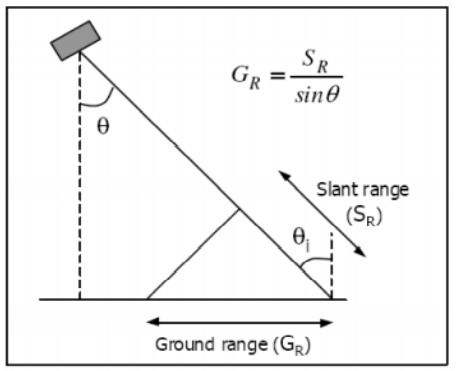
\includegraphics[height=12em]{pic/chap01xx07.jpg}
    \caption{斜距地距}
    \label{fig:0108}
\end{figure}


\begin{itemize}
    \item 斜距(Slant range):雷达到目标的距离方向, 雷达探测斜距方向的回波信号
    \item 地距(Ground range):将斜距投影到地球表面, 是地面物体间的真实距离
\end{itemize}
相同距离的地物, 地距相等, 但是由于入射角不同, 所以斜距不同, 导致雷达斜距图像上的近距离压缩, 就是图像失真, 消除失真的方式就是采用地距的显示方式.

雷达成像中, 在距离向上是按照地物目标反射信息的先后记录成像的,在高程上即使微小变化都可造成相当大范围的扭曲, 这些诱导因子包括透视收缩(Foreshortening), 叠掩(Layover), 阴影(Shadow). 如下图所示: 点 a, b和c在斜距表面成像为点 a', b'和 c'.由于地形的影响,在图像上三个点的顺序发生了变化, 如图\ref{fig:0109}所示.
\begin{figure}[htbp]
    \centering
    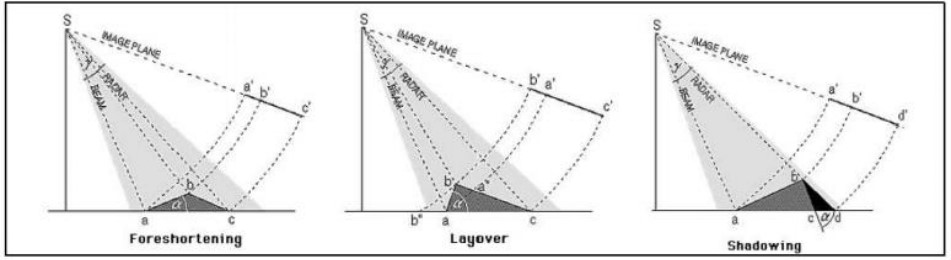
\includegraphics[height=10em]{pic/chap01xx09.jpg}
    \caption{透视收缩, 叠掩, 阴影}
    \label{fig:0109}
\end{figure}